\chapter{Implementation}\label{cha:implementation}

The \gls{FFT} application has been implemented in {\CPP}, {\CU}, {\OCL}, {\DX}, and {\GL}. The application was tested on a {\NVCARD} and a {\AMDCARD} graphics card and on an {\INTELCPU}.

\section{Benchmark application GPU}

\subsection{FFT}

\subsubsection{Setup}

The implementation of the \gls{FFT} algorithm on a \gls{GPU} can be broken down into steps, see figure \ref{fig:algorithm-overview} for a simplified overview. The application setup differs among the tested technologies, however some steps can be generalized; get platform and device information, allocate device buffers and upload data to device.
\begin{figure}
	\centering
	\includestandalone[width=\textwidth]{figures/overview}
	\caption{Overview of the events in the algorithm.}
	\label{fig:algorithm-overview}
\end{figure}

The next step is to calculate the specific \gls{FFT} arguments for a $N$-point sequence for each \gls{kernel}. The most important differences between devices and platforms are local memory capacity and thread and block configuration. \Glspl{thread} per block was selected for the best performance. See table \ref{tab:threads-per-block} for details.
\begin{table}
	\centering
	\includestandalone[width=\textwidth]{tables/threadsperblock}
	\caption{Shared memory size in bytes, threads and block configuration per device.}
	\label{tab:threads-per-block}
\end{table}

\subsubsection{Thread and block scheme}

The threading scheme was one butterfly per thread, so that a sequence of sixteen points require eight threads. Each platform was configured to a number of threads per block (see table \ref{tab:threads-per-block}): any sequences requiring more butterfly operations than the threads per block configuration needed the computations to be split over several blocks. In the case of a sequence exceeding one block, the sequence is mapped over the \code{blockIdx.y} dimension with size \code{gridDim.y}. The block dimensions are limited to $2^{31}$, $2^{16}$, $2^{16}$ respectively for \code{x}, \code{y}, \code{z}. Example: if the threads per block limit is two, then four blocks would be needed for a sixteen point sequence.

\begin{figure}
	% FFT Butterfly
\tikzstyle{n}= [circle, fill, minimum size=4pt,inner sep=0pt, outer sep=0pt]
\tikzstyle{mul} = [circle,draw,inner sep=-1pt]

% Define two helper counters
\newcounter{x}\newcounter{y}
\begin{tikzpicture}[%
	yscale=0.6,
	xscale=1.15,
	node distance=0.25cm,
	auto]
    % The strategy is to create nodes with names: N-column-row
    % Input nodes are named N-0-0 ... N-0-15
    % Output nodes are named N-10-0 ... N-10-15

    % Draw inputs
    \foreach \y in {0,...,15}
        \node[n, pin={[pin edge={latex'-,black}]left:$x(\y)$}] (N-0-\y) at (0,-\y) {};
              
    % Draw outputs
    \foreach \y in {0,...,15}
        \node[n, pin={[pin edge={-latex',black}]right:$X(\y)$}] (N-11-\y) at (8,-\y) {};
              
   % draw connector nodes
    \foreach \y in {0,...,15}
        \foreach \x / \c in {1/1,2/3,3/4,4/6,5/7,6/9,7/10}
            \node[n, name=N-\c-\y] at (\x,-\y) {};
            
    % draw x nodes
    \foreach \y in {0,...,7}
        \foreach \x / \c  in {1/2}
            \node[mul, right of=N-\x-\y] (N-\c-\y) {};            
    \foreach \y in {8,...,15}
        \foreach \x / \c  in {1/2}
            \node[mul, right of=N-\x-\y] (N-\c-\y) {${\times}$};
    % 
    \foreach \y in {0,...,3}
        \foreach \x / \c  in {4/5}
            \node[mul, right of=N-\x-\y] (N-\c-\y) {};
    \foreach \y in {4,...,7}
        \foreach \x / \c  in {4/5}
            \node[mul, right of=N-\x-\y] (N-\c-\y) {${\times}$};
    \foreach \y in {8,...,11}
        \foreach \x / \c  in {4/5}
            \node[mul, right of=N-\x-\y] (N-\c-\y) {};
    \foreach \y in {12,...,15}
        \foreach \x / \c  in {4/5}
            \node[mul, right of=N-\x-\y] (N-\c-\y) {${\times}$};
    % 
    \foreach \y in {0,2,4,6,8,10,12,14}
        \foreach \x / \c  in {7/8}
            \node[mul, right of=N-\x-\y] (N-\c-\y) {};
    \foreach \y in {1,3,5,7,9,11,13,15}
        \foreach \x / \c  in {7/8}
            \node[mul, right of=N-\x-\y] (N-\c-\y) {${\times}$};    

    % horizontal connections
    % Note the use of simple counter arithmetics to get correct
    % indexes.
    \foreach \y in {0,...,15}
    {
		\foreach \x in {0,1,3,4,7}
		{
			\setcounter{x}{\x}\stepcounter{x}
			\path (N-\x-\y) edge[-] (N-\arabic{x}-\y);
		}
	}
       
    % Draw the W_16 coefficients
    \setcounter{y}{0}
    \foreach \i in {0,...,7}
    {
	   	\path (N-2-\arabic{y}) edge[-] node {} (N-3-\arabic{y});
	    \stepcounter{y}
    }
    \foreach \i in {0,...,7}
    {
    	\path (N-2-\arabic{y}) edge[-] node {\tiny $W^{\i}_{16}$} (N-3-\arabic{y});
        \stepcounter{y}
    }
    
    % Draw the W_8 coefficients
    \setcounter{y}{0}
    \foreach \tmp in {0,1}
	{
    	\foreach \i in {0,...,3}
    	{
        	\path (N-5-\arabic{y}) edge[-] node {} (N-6-\arabic{y});
        	\addtocounter{y}{1}
    	}
    	\foreach \i in {0,...,3}
    	{
        	\path (N-5-\arabic{y}) edge[-] node {\tiny $W^{\i}_{8}$} (N-6-\arabic{y});
        	\addtocounter{y}{1}
    	}
    }

    % Draw the W_4 coefficients
    \setcounter{y}{0}
	\foreach \tmp in {0,...,3}
	{    
		\foreach \i in {0,1}
		{
			\path (N-8-\arabic{y}) edge[-] node {} (N-9-\arabic{y});
			\stepcounter{y}
			\path (N-8-\arabic{y}) edge[-] node {\tiny $W^{\i}_{4}$} (N-9-\arabic{y});
			\stepcounter{y}
		}
    }
    
    % Connect nodes
    \foreach \sourcey / \desty in {	0/8,	1/9,	2/10,	3/11,
									4/12,	5/13,	6/14,	7/15,
									8/0,	9/1,	10/2,	11/3,
									12/4,	13/5,	14/6,	15/7}
       \path (N-0-\sourcey.east) edge[-] (N-1-\desty.west);
    \foreach \sourcey / \desty in {	0/4,	1/5,	2/6,	3/7,
									4/0,	5/1,	6/2,	7/3,
									8/12,	9/13,	10/14,	11/15,
									12/8,	13/9,	14/10,	15/11}
        \path (N-3-\sourcey.east) edge[-] (N-4-\desty.west);
    \foreach \sourcey / \desty in {	0/0,	1/2,	2/0,	3/2,
    								0/1,	1/3,	2/1,	3/3,
                                   	4/4,	5/6,	6/4,	7/6,
                                   	4/5,	5/7,	6/5,	7/7,
                                   	8/8,	9/10,	10/8,	11/10,
									8/9,	9/11,	10/9,	11/11,
									12/12,	13/14,	14/12,	15/14,
									12/13,	13/15,	14/13,	15/15}
	{
        \path (N-6-\sourcey.east) edge[-] (N-7-\desty.west);
        \path (N-9-\sourcey.east) edge[-] (N-10-\desty.west);
    }
    % Nodes are in bit-reverse order
    \foreach \sourcey / \desty in {	0/0,1/8,2/4,3/12,4/2,5/10,6,7/14,8/1,9,10/5,11/13,12/3,13/11,14/7,15/15}
	{
        \path (N-10-\sourcey.east) edge[-] (N-11-\desty.west);
    }
    
    % Add region boxes
	% Partial stage
	\def \lastNode {10}
	\node[draw,dashed,fit=(N-6-0) (N-\lastNode-3)] {};
	\node[draw,dashed,fit=(N-6-4) (N-\lastNode-7)] {};
	\node[draw,dashed,fit=(N-6-8) (N-\lastNode-11)] {};
	\node[draw,dashed,fit=(N-6-12) (N-\lastNode-15)] {};	
    % Complete stage
	\node[draw,densely dotted,fit=(N-0-0) (N-2-15),label=above:{stage 1}] {};
	\node[draw,densely dotted,fit=(N-3-0) (N-5-15),label=above:{stage 2}] {};
	\node[draw,fit=(N-6-0) (N-8-15),opacity=0,label=above:{stage 3},name=Stage-3] {};
	\node[draw,fit=(N-9-0) (N-\lastNode-15),opacity=0,label=above:{stage 4},name=Stage-4] {};
	\node[draw,fit=(N-11-0) (N-11-15),opacity=0,label=above:{output}] {};
	\node[draw,densely dotted,fit=(Stage-3) (Stage-4)] {};
	\node[draw,fit=(N-\lastNode-0) (N-11-15)] {};
\end{tikzpicture}
	\caption{Flow graph of a 16-point FFT using (stage 1 and 2) {\CTALG} algorithm and (stage 3 and 4) constant geometry algorithm. The solid box is the bit-reverse order output. Dotted boxes are separate kernel launches, dashed boxes are data transfered to local memory before computing the remaining stages.}
	\label{fig:flowgraph-16}
\end{figure}

\subsubsection{Synchronization}

\Gls{thread} synchronization is only available of \glspl{thread} within a \gls{block}. When the sequence or partial sequence fitted within a block, that part was transferred to local memory before computing the last stages. If the sequence was larger and required more than one block, the synchronization was handled by launching several kernels in the same stream to be executed in sequence. The kernel launched for block wide synchronization is called the \emph{global kernel} and the kernel for thread synchronization within a block is called the \emph{local kernel}. The global kernel had an implementation of the {\CTALG} \gls{FFT} algorithm, and the local kernel had constant geometry (same indexing for every stage). The last stage outputs data from the shared memory in bit-reversed order to the global memory. See figure \ref{fig:flowgraph-16}, where the sequence length is 16 and the threads per block is set to two.

\subsubsection{Calculation}

The indexing for the global kernel was calculated from the thread id and block id (\code{threadIdx.x} and \code{blockIdx.x} in CUDA) as seen in figure \ref{fig:code-global-index}. Input and output is located by the same index.
\begin{figure}
	\centering
	\lstset{language=C++}
	\begin{framed}
	\begin{lstlisting}
int tid     = blockIdx.x * blockDim.x + threadIdx.x,
    io_low  = tid + (tid & (0xFFFFFFFF << stages_left)),
    io_high = io_low + (N >> 1);
	\end{lstlisting}
	\end{framed}
	\caption{ {\CU} example code showing index calculation for each stage in the global kernel, N is the total number of points. \code{io\_low} is the index of the first input in the butterfly operation and \code{io\_high} the index of the second.}
	\label{fig:code-global-index}
\end{figure}

Index calculation for the local kernel is done once for all stages, see figure \ref{fig:code-local-index}. These indexes are separate from the indexing in the global memory. The global memory offset depends on threads per block (\code{blockDim.x} in {\CU}) and block id.
\begin{figure}
	\centering
	\lstset{language=C++}
	\begin{framed}
	\begin{lstlisting}
int n_per_block = N / gridDim.x.
    in_low      = threadId.x.
    in_high     = threadId.x + (n_per_block >> 1).
    out_low     = threadId.x << 1.
    out_high    = out_low + 1;
	\end{lstlisting}
	\end{framed}
	\caption{ {\CU} code for index calculation of points in shared memory. }
	\label{fig:code-local-index}
\end{figure}

The last operation after the last stage is to perform the bit-reverse indexing operation, this is done when writing from shared to global memory. The implementation of bit-reverse is available as an intrinsic integer instruction (see table \ref{tab:bit-reverse-intrinsics}). If the bit-reverse instruction is not available, figure \ref{fig:code-bit-reverse} shows the code used instead. The bit-reversed value had to be right shifted the number of zeroes leading the number in a 32-bit integer type value. Figure \ref{fig:flowgraph-16} show the complete bit-reverse operations of a 16-point sequence in the output step after the last stage.

\begin{table}
	\centering
	\includestandalone[width=\textwidth]{tables/bit-reverse-intrinsics}
	\caption{Integer intrinsic bit-reverse function for different technologies.}
	\label{tab:bit-reverse-intrinsics}
\end{table}

\begin{figure}
	\centering
	\lstset{language=C++}
	\begin{framed}
	\begin{lstlisting}
x = (((x & 0xaaaaaaaa) >> 1) | ((x & 0x55555555) << 1));
x = (((x & 0xcccccccc) >> 2) | ((x & 0x33333333) << 2));
x = (((x & 0xf0f0f0f0) >> 4) | ((x & 0x0f0f0f0f) << 4));
x = (((x & 0xff00ff00) >> 8) | ((x & 0x00ff00ff) << 8));
return((x >> 16) | (x << 16));
	\end{lstlisting}
	\end{framed}
	\caption{ Code returning a bit-reversed unsigned integer where x is the input. Only 32-bit integer input and output. }
	\label{fig:code-bit-reverse}
\end{figure}

\subsection{FFT 2D}

\begin{figure}
	\centering
	\subfloat[Original image\label{image-1:lena}]{
		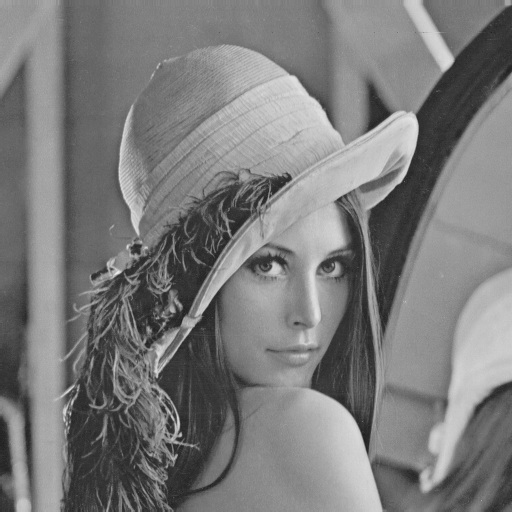
\includegraphics[keepaspectratio=true, scale=0.33]{images/lena.jpg}{}		
    }
    \hfill
    \subfloat[Magnitude representation\label{image-2:lena}]{
		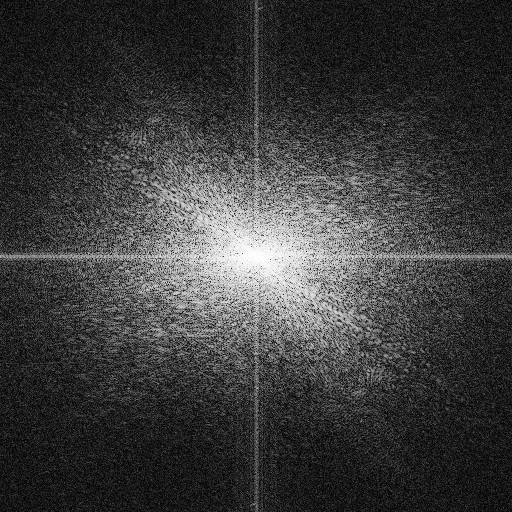
\includegraphics[keepaspectratio=true, scale=0.33]{images/lena_transformed.jpg}{}
    }
	\caption{Original image in \ref{image-1:lena} transformed and represented with a quadrant shifted magnitude visualization (scale skewed for improved illustration) in \ref{image-2:lena}. }
    \label{fig:twodimentransform}
\end{figure}

The \gls{FFT} algorithm for \gls{2D} data, such as images, is first transformed row-wise (each row as a separate sequence) and then an equal transform of each column. The application performs a row-wise transformation followed by a transpose of the image to reuse the row-wise transform procedure for the columns. This method gives better memory locality when transforming the columns. A transformed image is shown in figure \ref{fig:twodimentransform}.

The difference between the \gls{FFT} kernel for \gls{1D} and \gls{2D} is the indexing scheme. \gls{2D} rows are indexed with \code{blockIdx.x}, and columns with \code{threadIdx.x} added with an offset of \code{blockIdx.y} $\cdot$ \code{blockDim.x}.

\subsubsection{Transpose}

The transpose kernel uses a different index mapping of the 2D-data and threads per blocks than the \gls{FFT} kernel. The data is tiled in a grid pattern where each tile represents one block, indexed by \code{blockIdx.x} and \code{blockIdx.y}. The tile size is a multiple of 32 for both dimensions and limited to the size of the shared memory buffer, see table \ref{tab:threads-per-block} for specific size per technology. To avoid banking issues, the last dimension is increased with one but not used. However, resolving the banking issue have little effect on total running-time so when shared memory is limited to 32768, the extra column is not used. The tile rows and columns are diveded over the \code{threadIdx.x} and \code{threadIdx.y} index respectively. See figure \ref{lst:cuda:device-transpose} for code example.

Shared memory example: The {\CU} shared memory can allocate 49152 bytes and a single data point require $\code{sizeof(float)} \cdot 2 = 8$ bytes. That leaves room for a tile size of $64 \cdot (64 + 1) \cdot 8 = 33280$ bytes. Where the integer $64$ is the highest power of two that fits.

\begin{figure}
	\centering
	\begin{framed}
		\includestandalone[width=\textwidth]{code/cuda-device-transpose}	
	\end{framed}
	\caption{CUDA device code for the transpose kernel.}
	\label{lst:cuda:device-transpose}	
\end{figure}

The transpose kernel uses the shared memory and tiling of the image to avoid large strides through global memory. Each block represents a tile in the image. The first step is to write the complete tile to shared memory and synchronize the threads before writing to the output buffer. Both reading from the input memory and writing to the output memory is performed in close stride. Figure \ref{fig:transpose-memory} shows how the transpose is performed in memory.

\begin{figure}
	\centering
	\includestandalone[width=\textwidth]{figures/transpose-tile}
	\caption{Illustration of how shared memory is used in transposing an image. Input data is tiled and each tile is written to shared memory and transposed before written to the output memory. }
	\label{fig:transpose-memory}
\end{figure}

\subsection{Differences}%
\subsubsection{Setup}%
The majority of differences in the implementations were related to the setup phase. The {\CU} implementation is the most straight forward, using \code{cudaMalloc(...)} to allocate a buffer and \code{cudaMemcpy(...)} to populate it. With {\CU} you can write the device code in the same file as the host code and share functions. {\OCL} and {\GL} require a \code{char *} buffer as the kernel source and is most practical if written in a separate file and read as a file stream to a \code{char} buffer. {\DX} shaders are most easily compiled from file. Figure \ref{fig:code:setup} gives a simplified overview of how to setup the kernels in the different technologies.%
\begin{figure}%
	\centering%
	\def \setupWidth {\textwidth / 2 - 18pt}%
	\subfloat[{\CU} setup\label{setup:cu}]{%
		\fbox{\includestandalone[width=\setupWidth]{code/setup/cu}}%
	}%
	\hfill%
	\subfloat[{\OCL} setup\label{setup:ocl}]{%
		\fbox{\includestandalone[width=\setupWidth]{code/setup/ocl}}%
	}%
	\vfill%
	\subfloat[{\DX} setup\label{setup:dx}]{%
		\fbox{\includestandalone[width=\setupWidth]{code/setup/dx}}%
	}%
	\hfill%
	\subfloat[{\GL} setup\label{setup:gl}]{%		
		\fbox{\includestandalone[width=\setupWidth]{code/setup/gl}}%
	}%
	\caption{An overview of the setup phase for the GPU technologies.}%
	\label{fig:code:setup}%
\end{figure}%

\subsubsection{Kernel execution}

Kernel execution in {\CU} is very much like any procedure execution in {\CPP} with the only difference that the kernel launch syntax $<<<$ and $>>>$ to set the block and thread dimension.

The other technologies require some more setup; {\OCL} and {\GL} need one function call per parameter. {\OCL} maps with index, whereas {\GL} maps with a string to the parameter. In {\DX} a constant buffer is suitable for the parameters. The constant buffer is read-only and accessible globally over the kernel. {\DX} and {\GL} share a similar launch style where the compute shader is set as the current program to the device context, and a dispatch call is made with the group (block) configuration. See table \ref{tab:kernel-execution} for a list of how the kernels are launched.

\begin{table}[H]
	\centering
	\includestandalone[width=\textwidth]{tables/kernel-execution}
	\caption{Table illustrating how to set parameters and launch a kernel.}
	\label{tab:kernel-execution}
\end{table}

\subsubsection{Kernel code}

This is the part where the code differ the least on but a few points. {\CU} have the strongest support for a {\CPP} -like language and only adds a function type specifier. The kernel program is accessible from the host via the \code{\_\_global\_\_} specifier. {\OCL} share much of this but restricted to a C99-style in the current version (2.0). One difference is how one can reference global and local buffers, these must be specified with the specifier \code{\_\_global} or \code{\_\_local}.

{\DX} and {\GL} Compute Shader is coded in \gls{HLSL} and \gls{GLSL} respectively. These languages are similar and share the same level of restrictions compared to CUDA C/C++ and {\OCL} C-code. Device functions can not use pointers or recursion. However these are of little importance for the performance since all code is in-lined in the compilation/building of the kernel program.

\subsubsection{Synchronization}

The synchronization of threads and blocks is slightly different, {\CU} have the options to synchronize threads within a block and to synchronize host and device, the equivalent exists in all but {\DX} where the device synchronization is not done trivially as with a blocking function call. {\CU}, {\OCL} and {\DX} uses the same kernel stream to execute kernels sequentially while in {\GL} the sequential execution is accomplished by the use of
\begin{lstlisting}
glMemoryBarrier(GL_SHADER_STORAGE_BARRIER_BIT)
\end{lstlisting}
in between launches. See table \ref{tab:kernel-synchronization} for the synchronization functions used.

\begin{table}[H]
	\centering
	\includestandalone[width={\textwidth}]{tables/kernel-synchronization}
	\caption{Synchronization in GPU technologies.}
	\label{tab:kernel-synchronization}
\end{table}

\section{Benchmark application CPU}

\subsection{FFT with OpenMP}

The {\OMP} implementation benefits in performance from calculating the twiddle factors in advance. The calculated values are stored in a buffer accessible from all threads. The next step is to calculate each stage of the \gls{FFT} algorithm. Last is the output index calculation where elements are reordered. See figure \ref{fig:omp:overview} for an overview.

\begin{figure}
	\centering
	\includestandalone[width=\textwidth]{figures/omp-overview}
	\caption{OpenMP implementation overview transforming sequence of size $N$.}
	\label{fig:omp:overview}
\end{figure}

\subsubsection{Twiddle factors}

The twiddle factor are stored for each butterfly operation. To save time, only the real part are calculated and the imaginary part is retrieved from the real parts due to the fact that $\sin(x) = \cos(\pi/2 + x)$ and $\sin(\pi/2 + x) = -\cos(x)$ to store. See figure \ref{tab:omp:twiddle-overview} for an example. The calculations will be split among the threads by static scheduling in two steps, first calculate the real values, secondly copy from real to imaginary.

\begin{table}
	\centering
	\begin{tabular}{|l|l|r|}
	\multicolumn{3}{c}{Table $W$} \\ \hline
	$i$ & $\Re(W)$ & $\Im(W)$ \\ \hline
	0 & $\cos(\alpha \cdot 0)$ & $\Re(W[4])$ \\
	1 & $\cos(\alpha \cdot 1)$ & $\Re(W[5])$ \\
	2 & $\cos(\alpha \cdot 2)$ & $\Re(W[6])$ \\
	3 & $\cos(\alpha \cdot 3)$ & $\Re(W[7])$ \\	
	4 & $\cos(\alpha \cdot 4)$ & $-\Re(W[0])$ \\
	5 & $\cos(\alpha \cdot 5)$ & $-\Re(W[1])$ \\
	6 & $\cos(\alpha \cdot 6)$ & $-\Re(W[2])$ \\
	7 & $\cos(\alpha \cdot 7)$ & $-\Re(W[3])$ \\ \hline
\end{tabular}
	\caption{Twiddle factors for a 16-point sequence where $\alpha$ equals $(2 \cdot \pi) / 16$. Each row $i$ corresponds to the $i$th butterfly operation.}
	\label{tab:omp:twiddle-overview}
\end{table}

\subsubsection{Butterfly}

The same butterfly operation uses the constant geometry index scheme. The indexes are not stored from one stage to the next but it makes the output come in continues order. The butterfly operations are split among the threads by static scheduling.

\subsubsection{Bit-Reversed Order}

See figure \ref{fig:omp:bit-reverse-order} for code showing the bit-reverse ordering operation in C/C++ code.

\begin{figure}
	\centering
	\begin{framed}
		\includestandalone[width=\textwidth]{code/omp-bit-reverse}	
	\end{framed}
	\caption{ C/C++ code performing the bit-reverse ordering of a N-point sequence. }
	\label{fig:omp:bit-reverse-order}
\end{figure}

\subsection{FFT 2D with OpenMP}

The implementation of \gls{2D} \gls{FFT} with {\OMP} run the transformations row-wise and transposes the image and repeat. The twiddle factors are calculated once and stays the same.

\subsection{Differences with GPU}

The OpenMP implementation differs from the \gls{GPU} with the fact that twiddle factors are pre computed and it uses the constant geometry implementation in all stages. The amount of parallel threads are on the {\INTELCPU} four whereas on the \gls{GPU} in the order of up to 192 (seven warps, one per \gls{SM}, with 32 threads each). This highly effects performance when the size of the problem grows.

\section{Benchmark configurations}

\subsection{Limitations}

All implementations are limited to handle sequences of $2^n$ length or $2^m \times 2^m$ where $n$ and $m$ are integers with maximal value of $n = m + m = 26$. The selected \gls{GPU}s have a maximum of 2GB global memory available. The limitation is required since the implementation uses a total of $2^{26} \cdot \code{sizeof(float2)} \cdot 2 = 1073741824$ bytes. However on the {\AMDCARD} card, problems with {\DX} and {\GL} set the limit lower. {\DX} handled sizes of $n <= 2^{24}$ and {\GL} $n <= 2^{24}$ and $m <= 2^{9}$.

\subsection{Testing}

All tests executed on the \gls{GPU} utilize some implementation of event time stamps. The time stamp event retrieve the actual start of the kernel if the current stream is busy. The \gls{CPU} implementations used Windows \emph{QueryPerformanceCounter} function, which is a high resolution ($<1{\micro}s$) time stamp.

\subsection{Reference libraries}

One reference libraries per platform was included to compare how well the FFT implementation performed. The \emph{\FFTW} library for the \gls{CPU}, runs a planning scheme to create an execution plan for each environment and data input size. Similar strategy is used in the {\CUFFT} and {\CLFFT} libraries used for the {\NVCARD} and {\AMDCARD} respectively. Table \ref{tab:external-implementations} sums up information about the external libraries.

\begin{table}
	\centering
	\begin{tabular}{|l|l|l|l|}
	\hline
	Platform & Model & Library name & Version \\ \hline
	NVIDIA GPU & GeForce GTX 670 & cuFFT & TODO \\
	AMD GPU & Radeon R7 260X & clFFT & 2.8.0 \\ \hline
	Intel CPU & Core i7 3770K 3.5GHz & FFTW & 3.3.4 \\ \hline
\end{tabular}
	\caption{Libraries included to compare with the implementation.}
	\label{tab:external-implementations}
\end{table}